\documentclass[12pt]{article}
\usepackage{graphicx}

\title{COP290: Complaint App}
\author{Bipul (2014cs50282) \\ Deepak (2014cs50435) \\ Shivank (2014cs10565) }

\begin{document}
\maketitle

We are developing a complaint management system which can be actively used in Institutes like IIT. Using this application, the end users can directly submit their complaint/grievance to the concerned authorities.

\section{User Interface}

\begin{figure}[!ht]
	\centering
	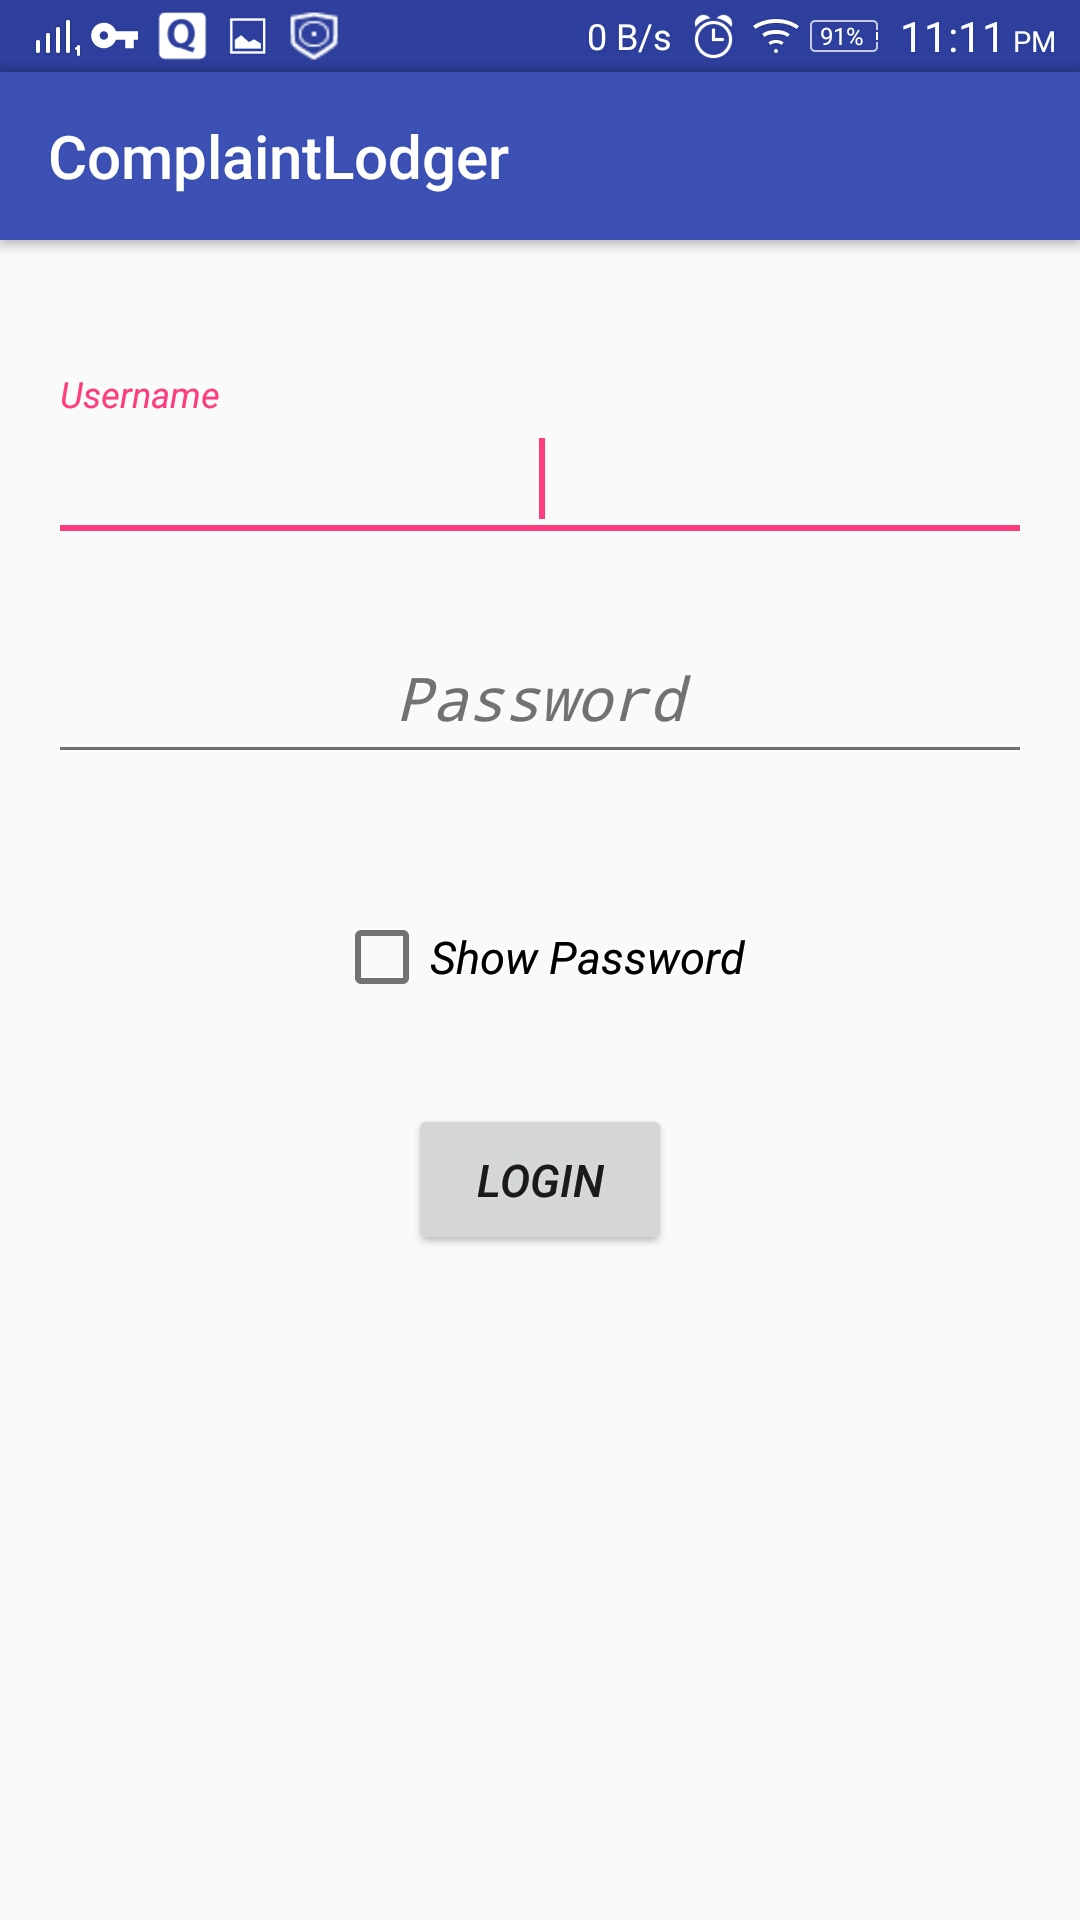
\includegraphics[width=0.5\textwidth]{login.jpeg}
	\caption{Login Screen}
\end{figure}
\begin{itemize}
    \item If user is loging in for the first time his password will be saved in database
\end{itemize}

\begin{figure}[!ht]
	\centering
	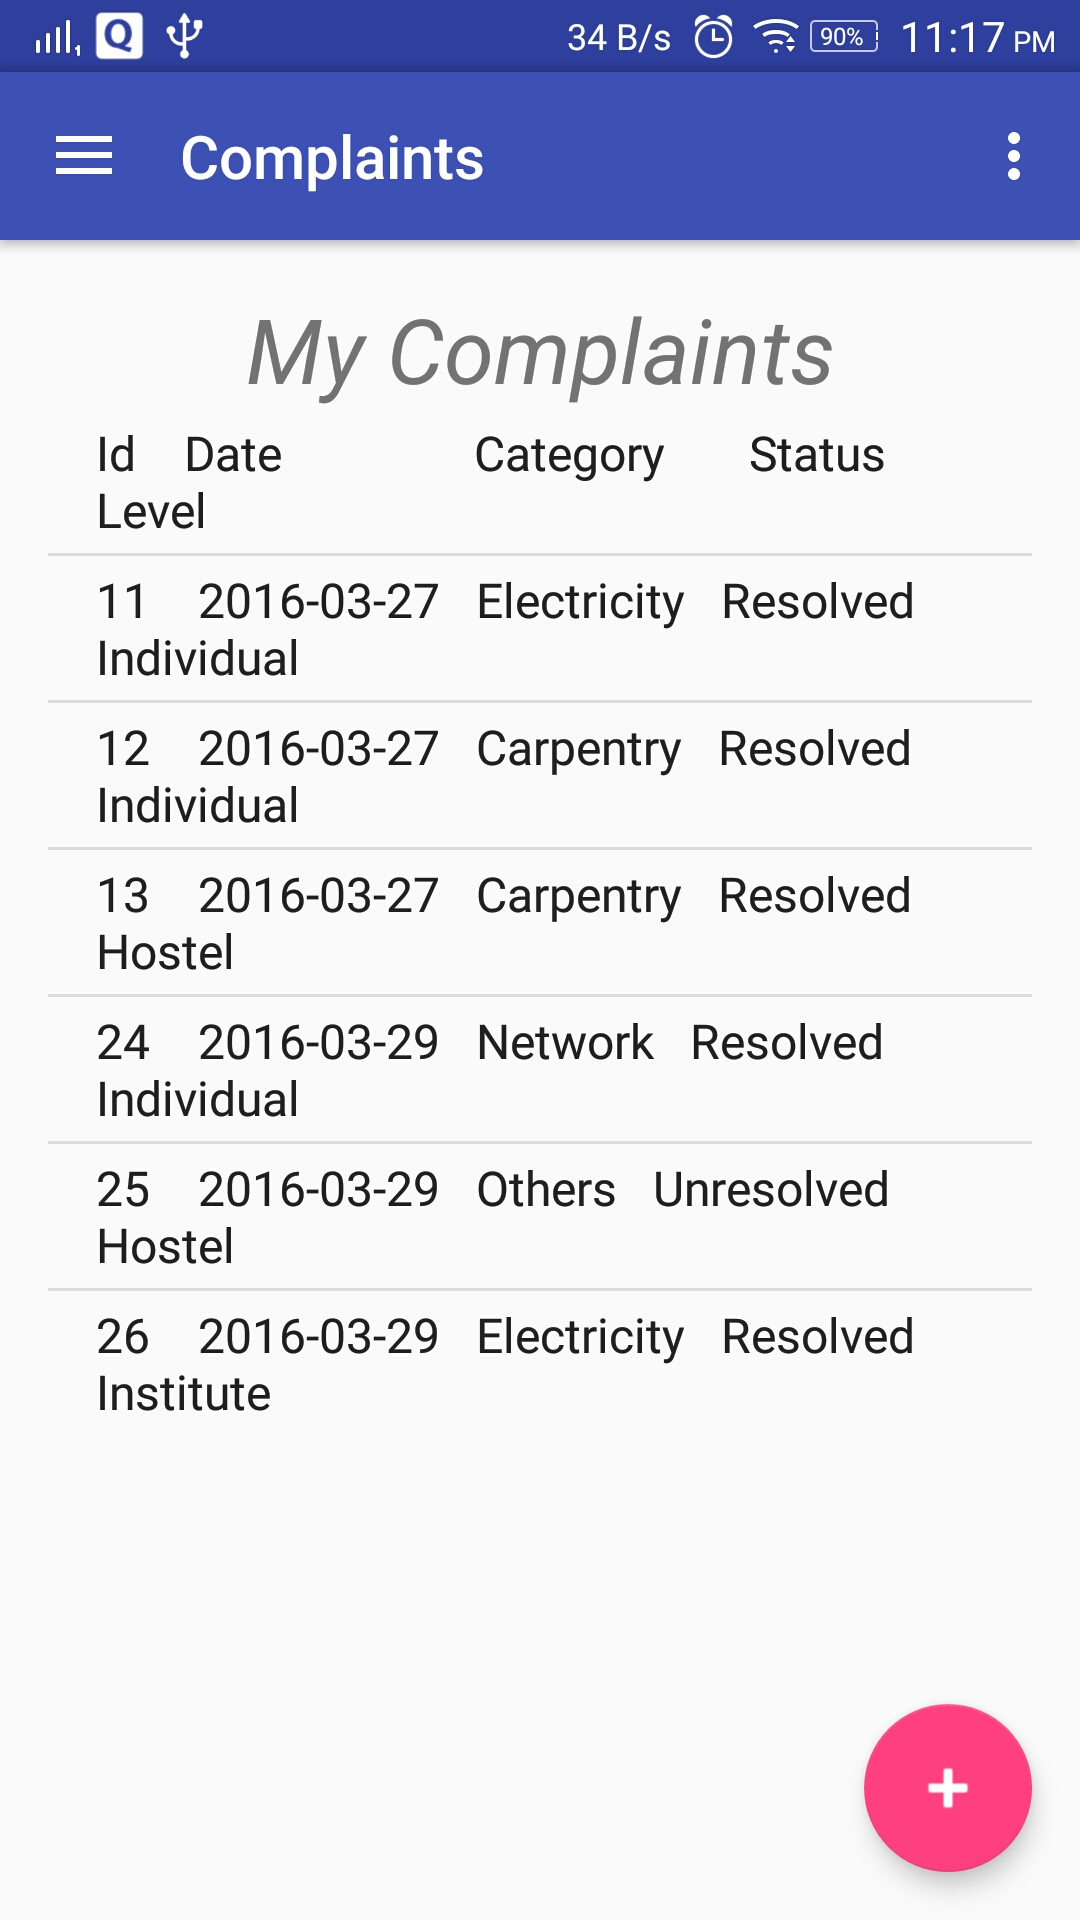
\includegraphics[width=0.5\textwidth]{welcome.jpeg}
	\caption{Main Page}
\end{figure}
\begin{itemize}
    \item It shows all the complaints related to him/his hostel/institute in list view.
    \item Private complaints has been marked by red circle, while hostel by green and Institute related complaints by Blue.
    \item Clicking on the top left corner brings navigation drawer through which he can directly access main links. 
    \item FAB has been given in almost every page so that user can report a complain immediately.
\end{itemize}

\begin{figure}[!ht]
	\centering
	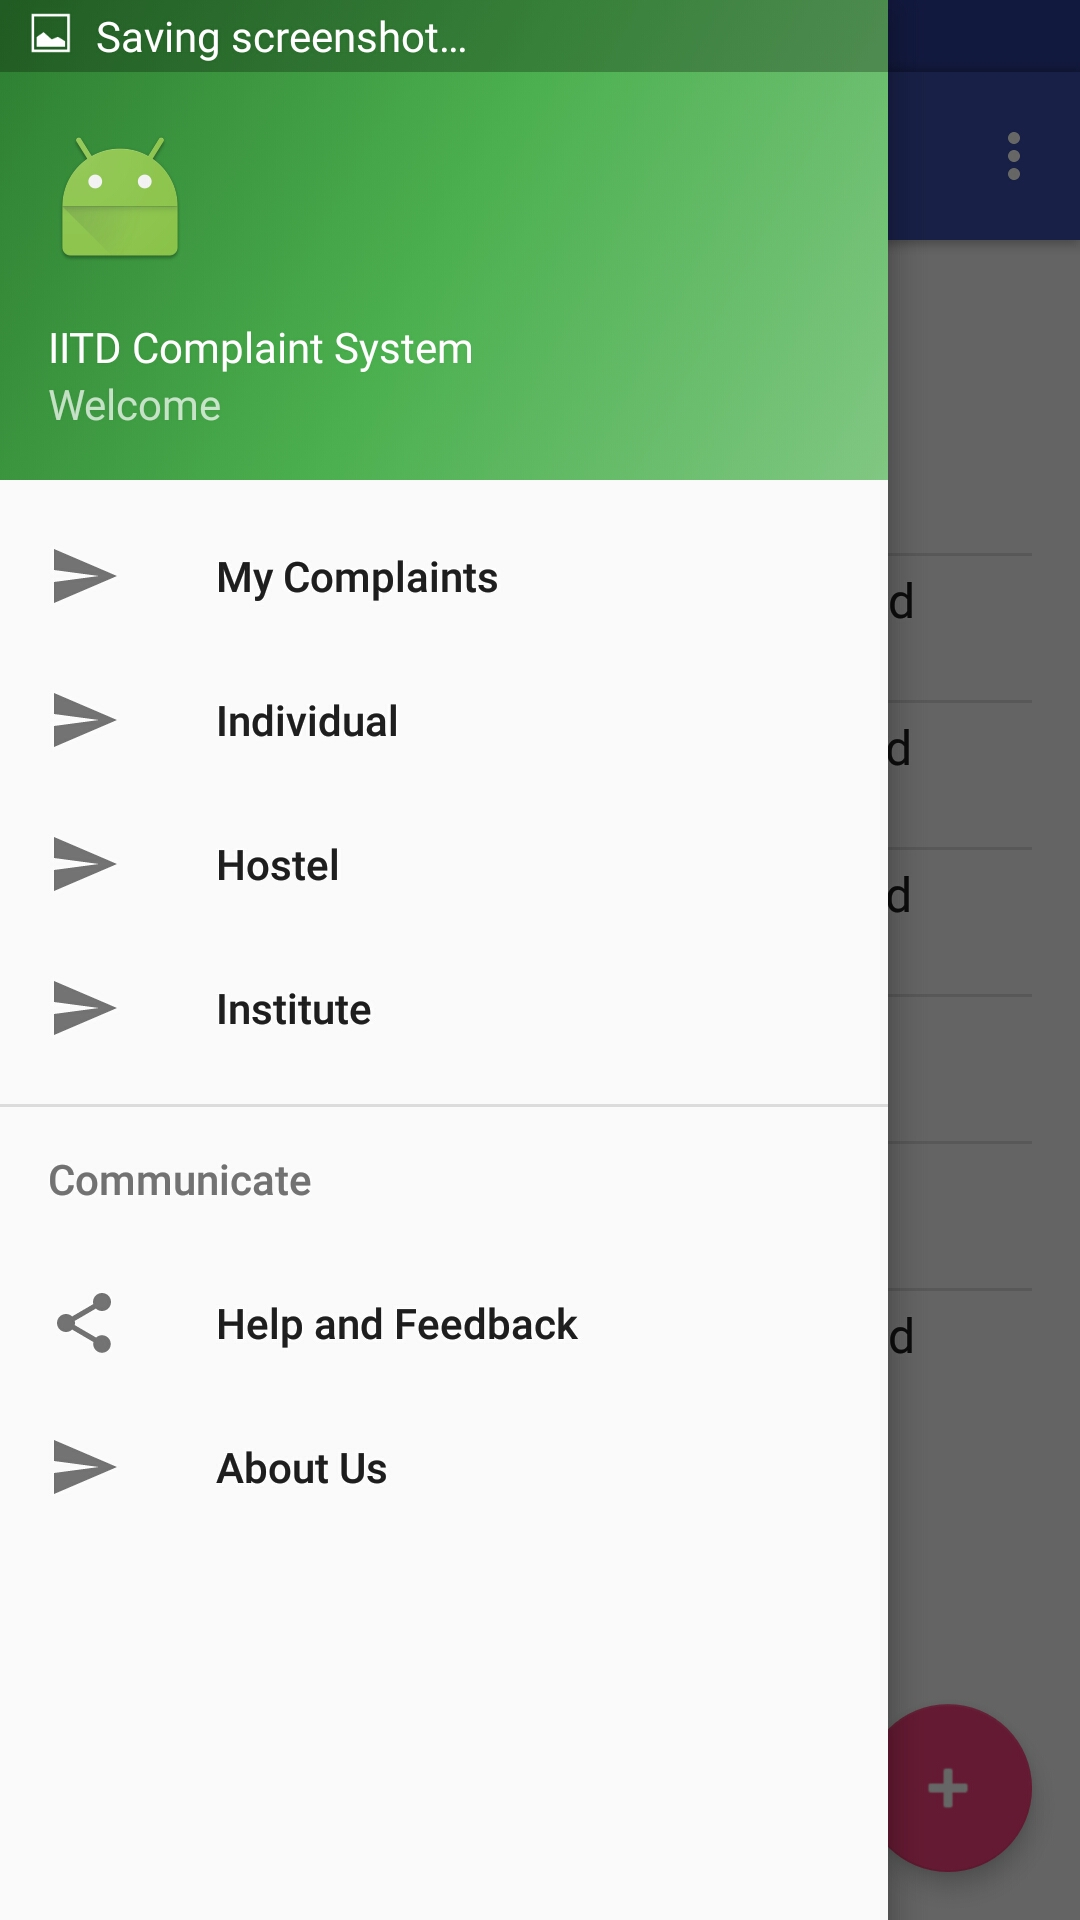
\includegraphics[width=0.5\textwidth]{drawer.jpeg}
	\caption{Navigation Drawer}
\end{figure}
\begin{itemize}
    \item Navigation Drawer holds a bunch of quick links to Bookmarked Complaints, His complaints, hostel and Institute related complaints.
\end{itemize}

\begin{figure}[!ht]
	\centering
	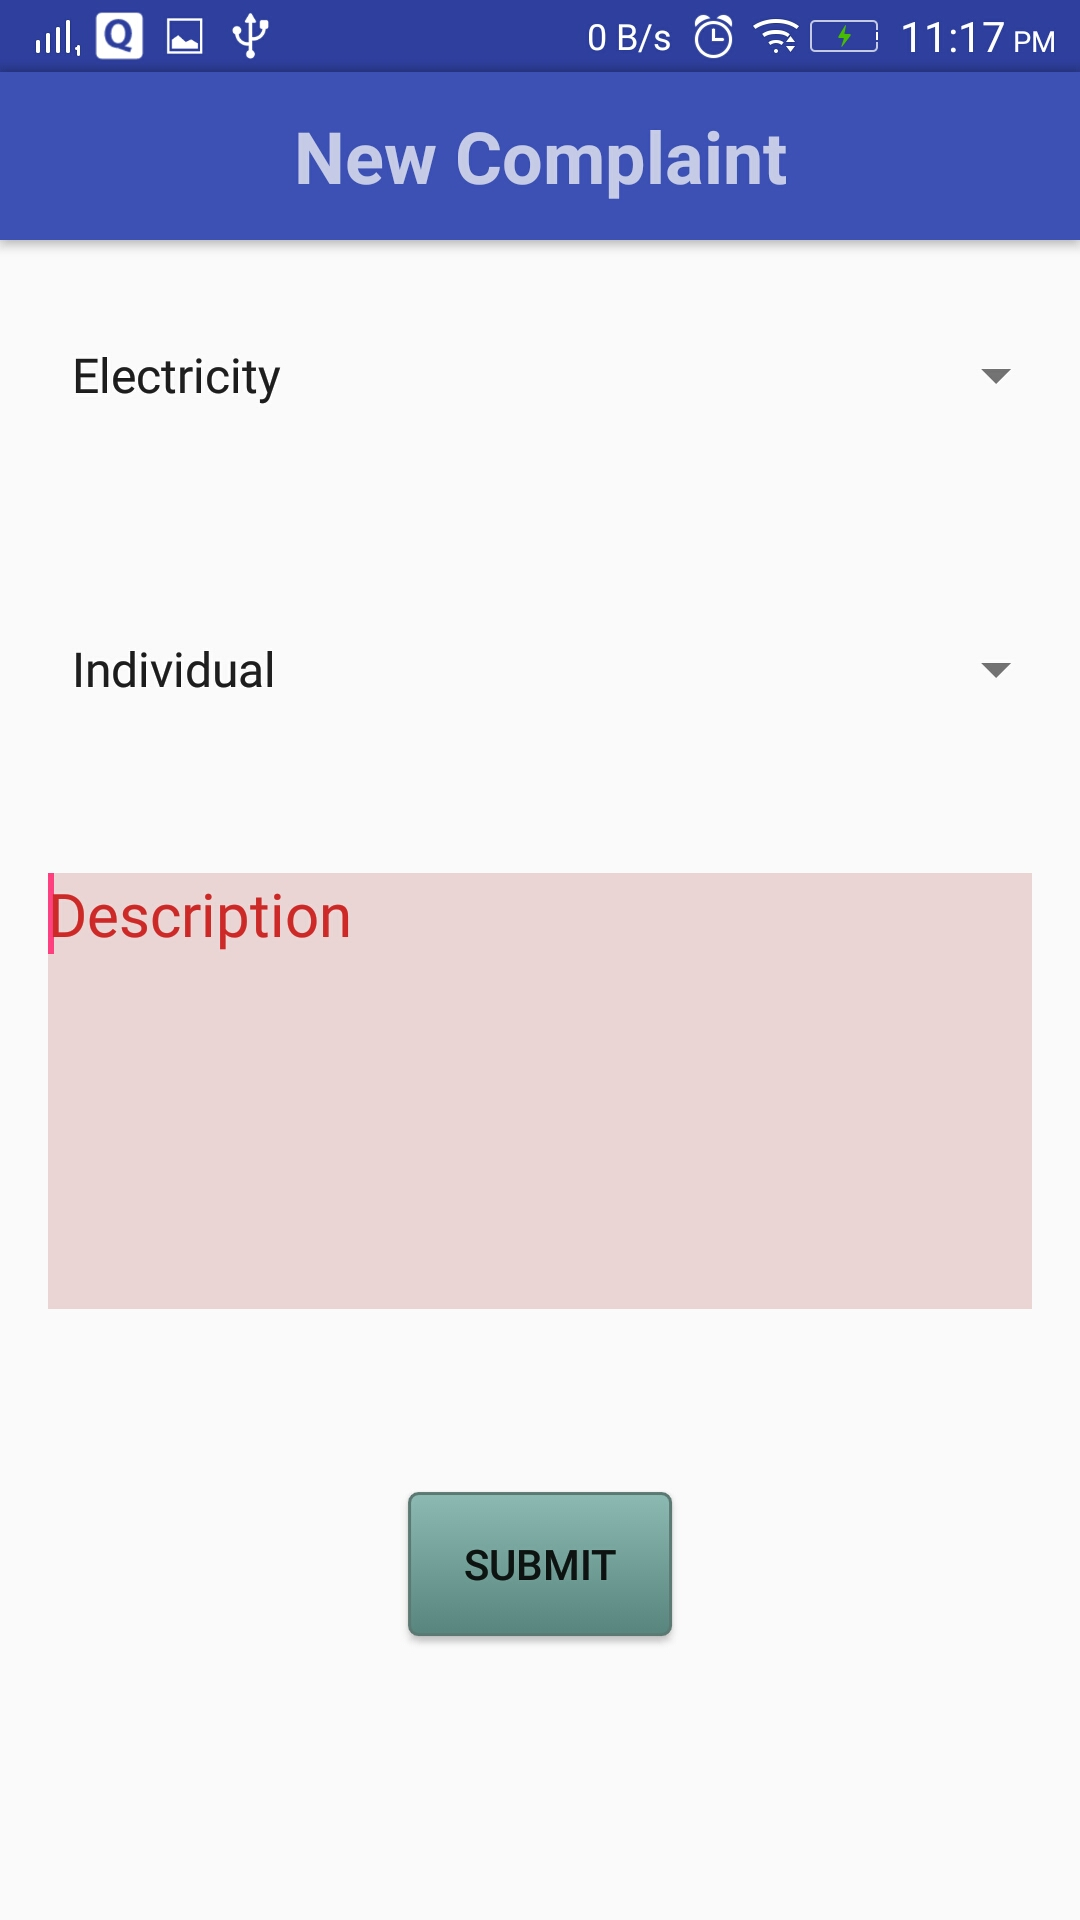
\includegraphics[width=0.5\textwidth]{addcomplaint.jpeg}
	\caption{New Complaint}
\end{figure}
\begin{itemize}
    \item Clicking on FAB brings out this page which holds a drop down menu for selecting category of complain.
    \item User fills up problem description and any comment like favourable time for rectification.
    \item Technician can use comment to tell any information related to the complaint.
\end{itemize}

\begin{figure}[!ht]
	\centering
	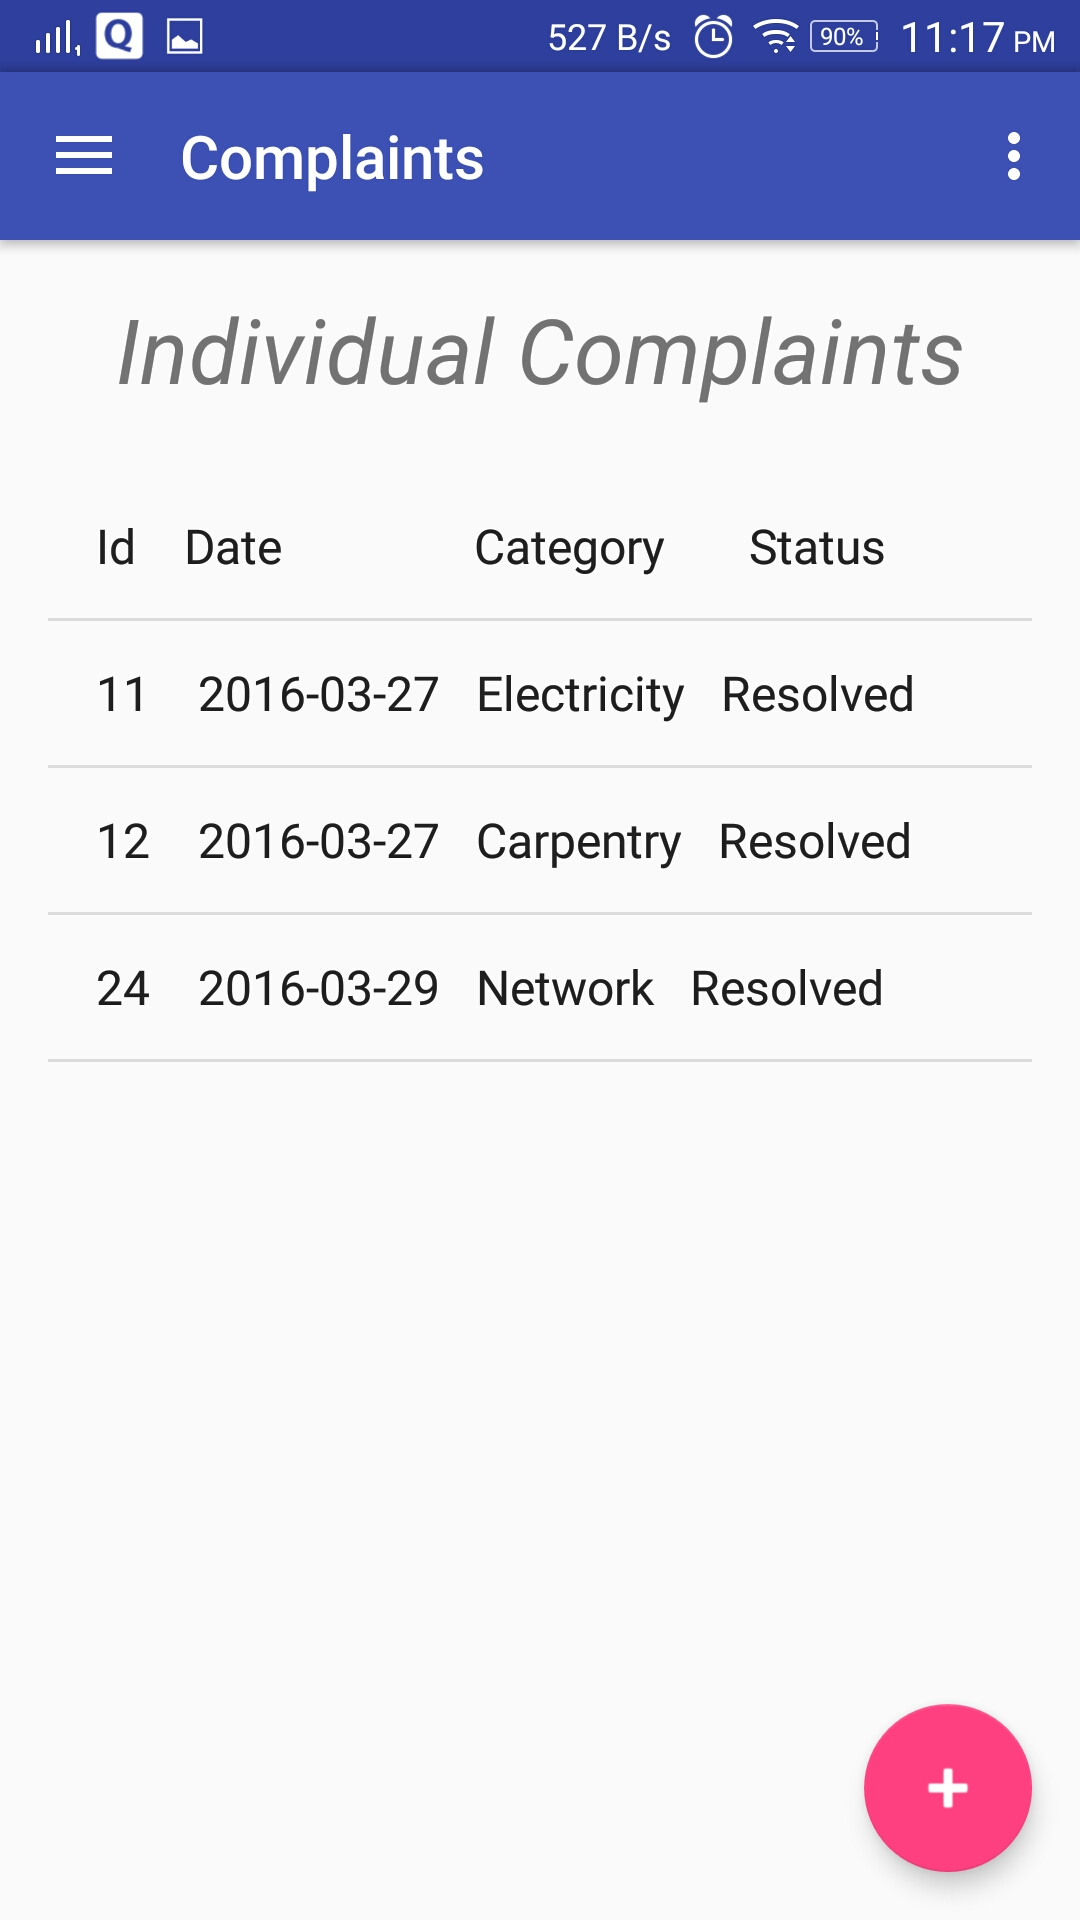
\includegraphics[width=0.5\textwidth]{indicomplaint.jpeg}
	\caption{Complaint Filed by User}
\end{figure}
\begin{itemize}
    \item This page shows all the personal complaints filed by the User, in list view with Fragment view to separate Unresolved and Resolved complaints.
    \item Clicking on any of the Problem in the list expands the list horizontally and show the complaint description including ticket ID, report Date, comments and option to mark Resolved or Unresolved.
\end{itemize}


\begin{figure}[!ht]
	\centering
	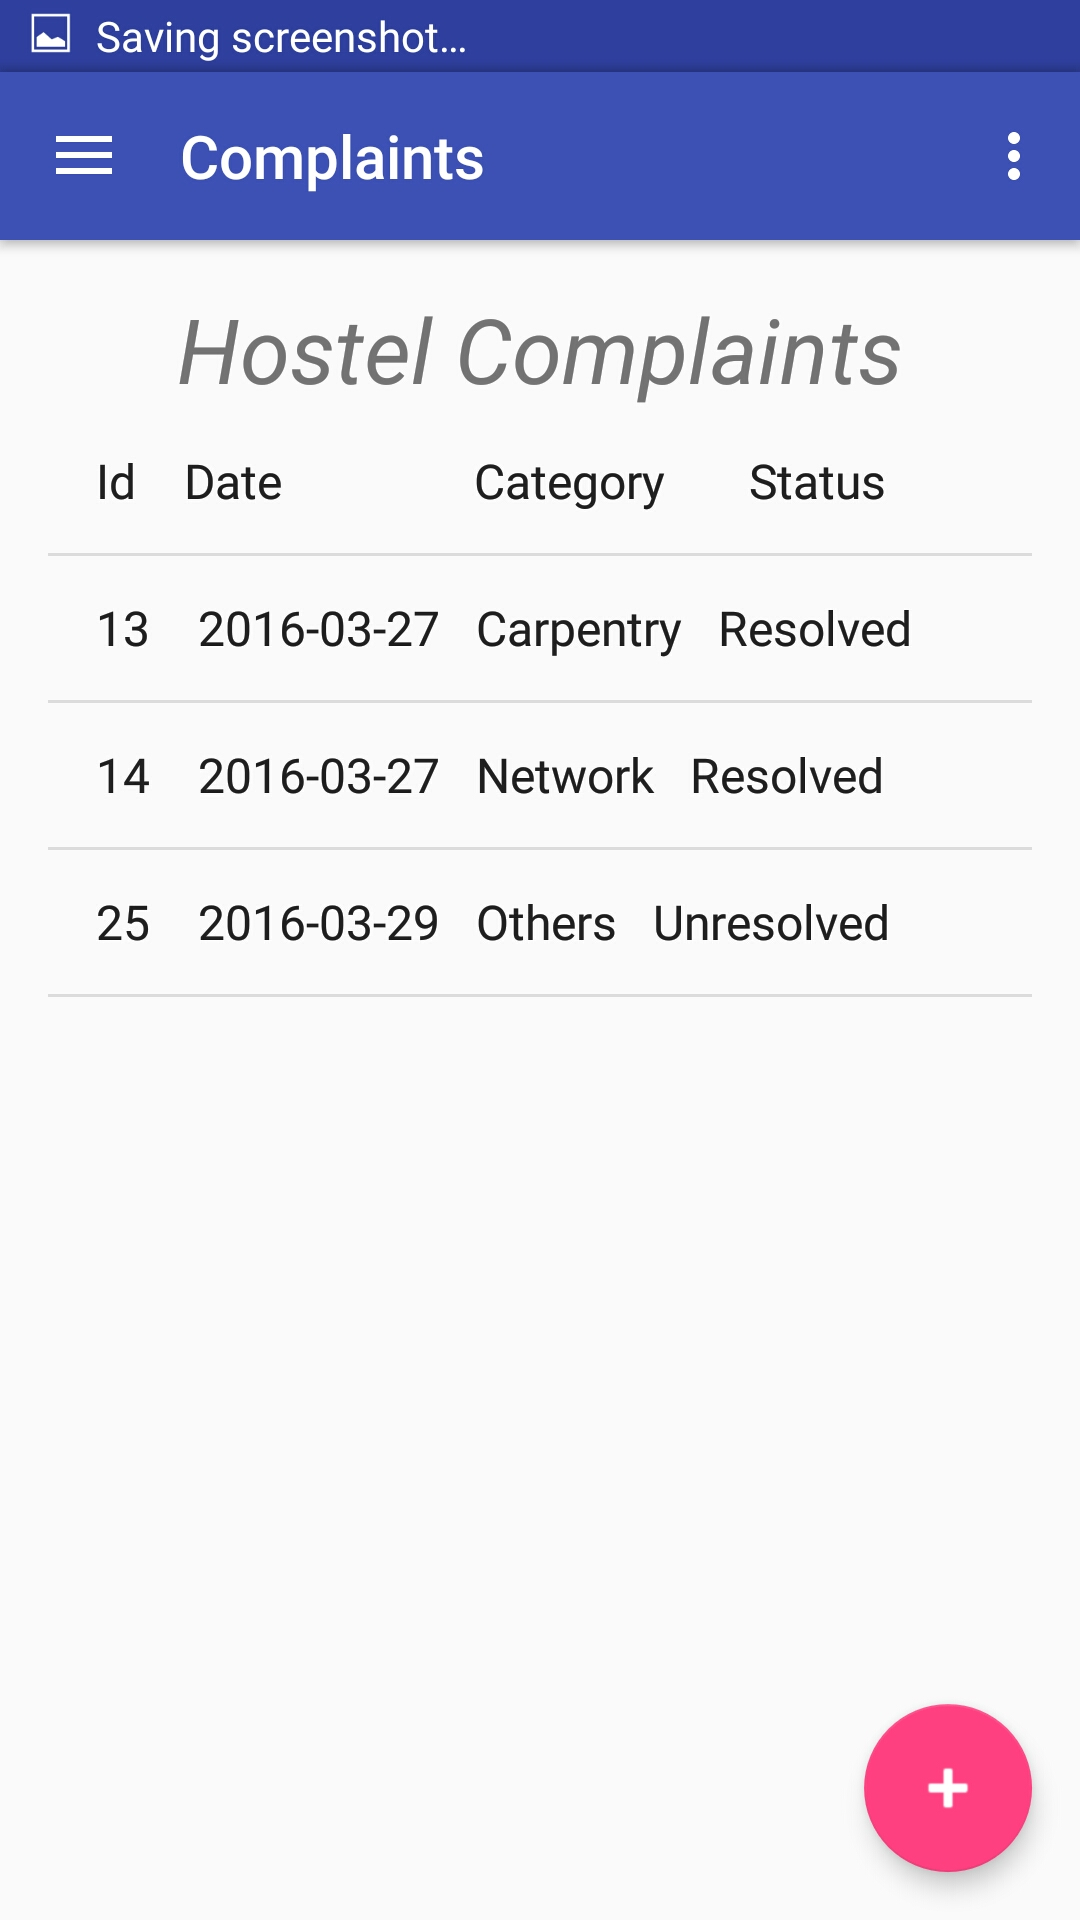
\includegraphics[width=0.5\textwidth]{hostelcomplaint.jpeg}
	\caption{Complaint Filed by Hostel}
\end{figure}
\begin{itemize}
    \item This page shows all the public complaints filed by the residents of hostel, in list view with Fragment view to separate Unresolved and Resolved complaints.
\end{itemize}

\begin{figure}[!ht]
	\centering
	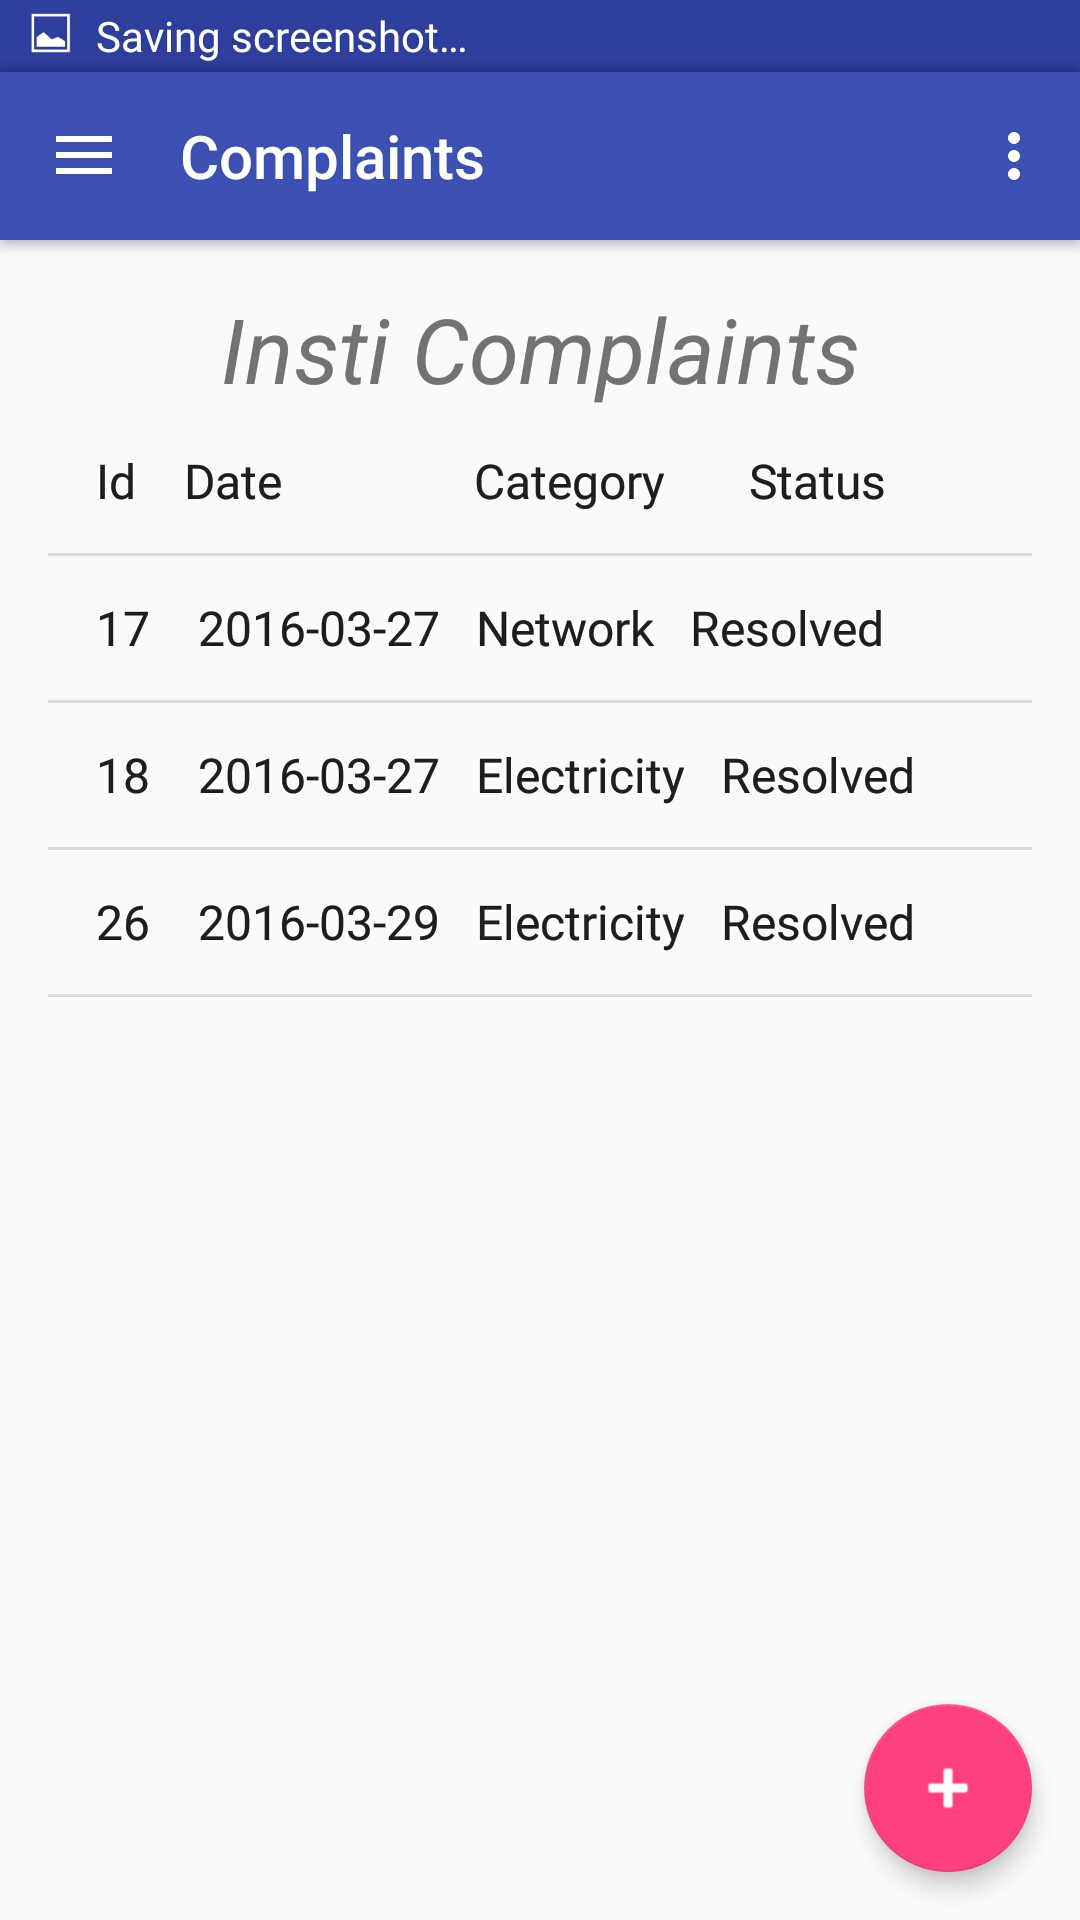
\includegraphics[width=0.5\textwidth]{insticomplaint.jpeg}
	\caption{Complaint Filed by Institute}
\end{figure}
\begin{itemize}
    \item This page shows all the public complaints filed by the residents of institute, in list view with Fragment view to separate Unresolved and Resolved complaints.
\end{itemize}


\begin{figure}[!ht]
	\centering
	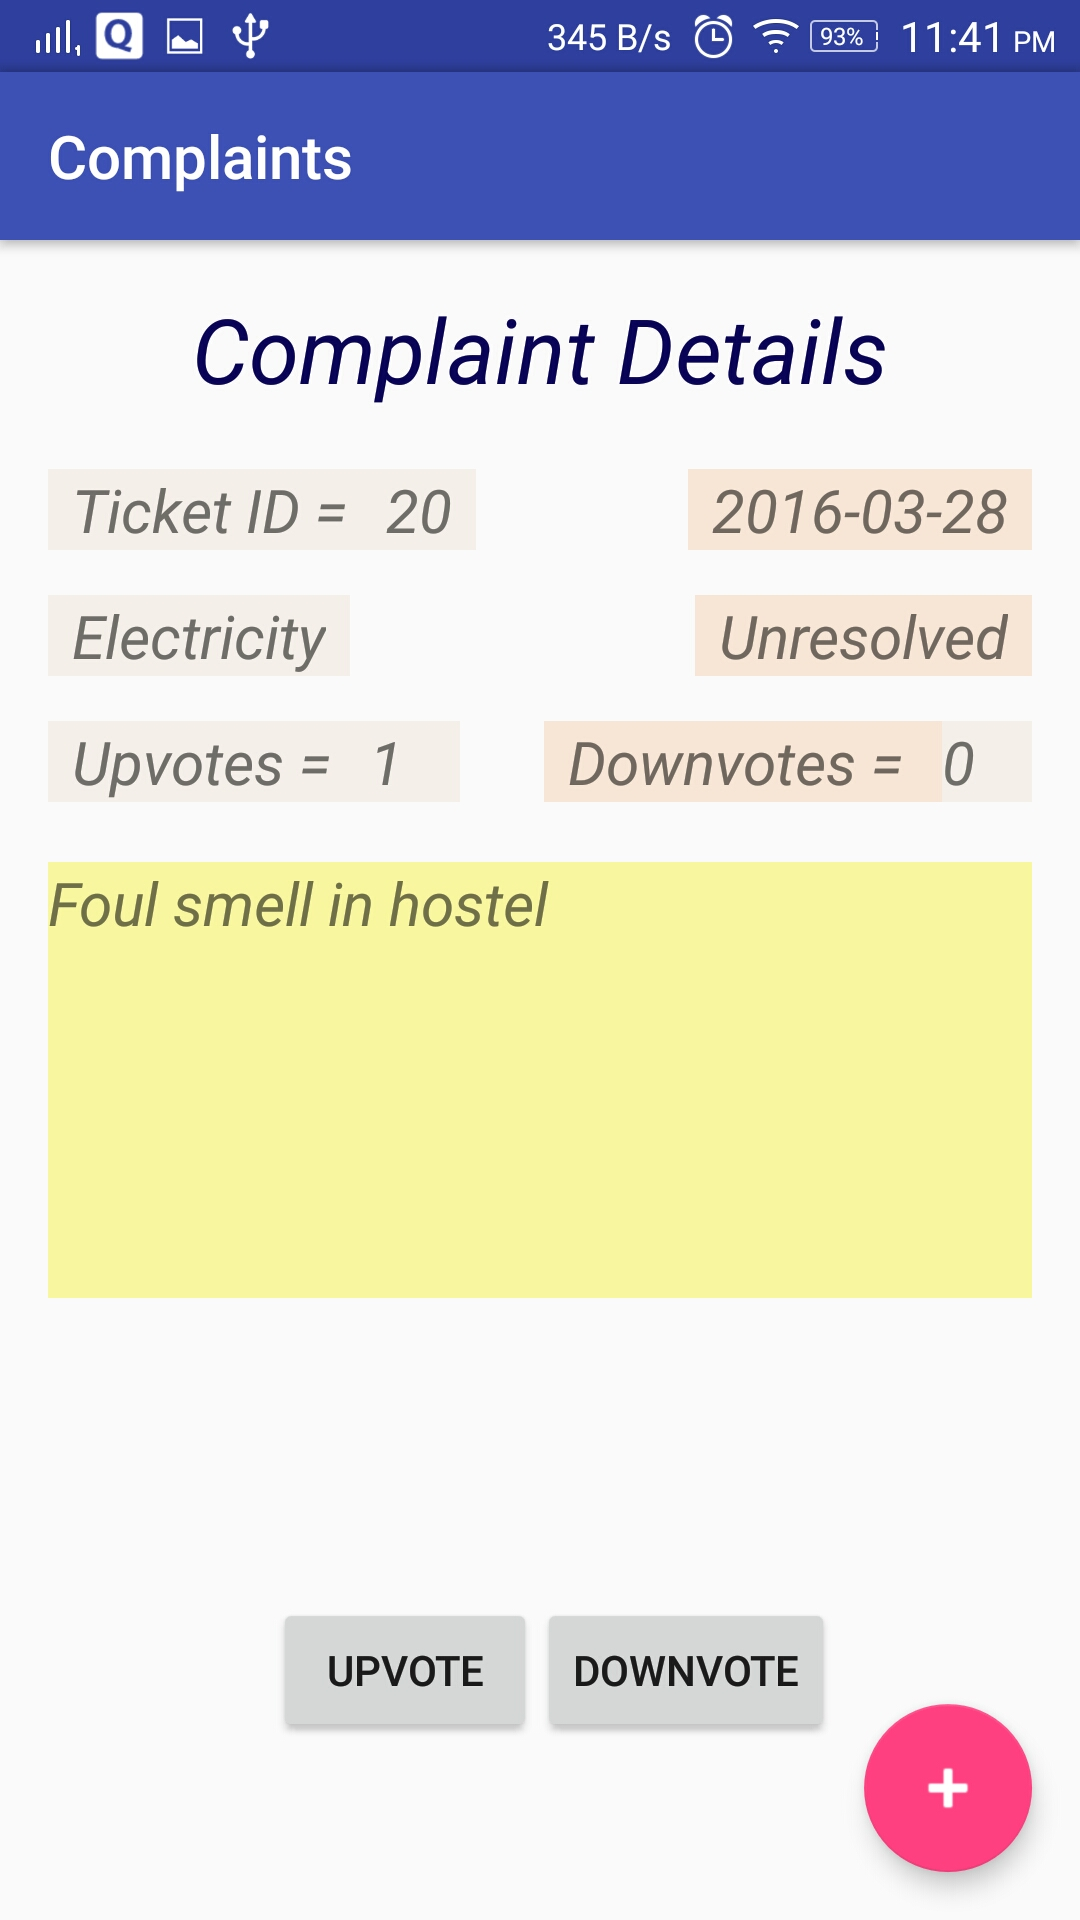
\includegraphics[width=0.5\textwidth]{description.jpeg}
	\caption{Complaint description}
\end{figure}
\begin{itemize}
    \item Clicking on any of the Problem in the list expands the list horizontally and show the complaint description including ticket ID, report Date, comments and option to Upvote and Downvote the Problem using Thumbs up and Thumbs down.
\end{itemize}

\begin{figure}[!ht]
	\centering
	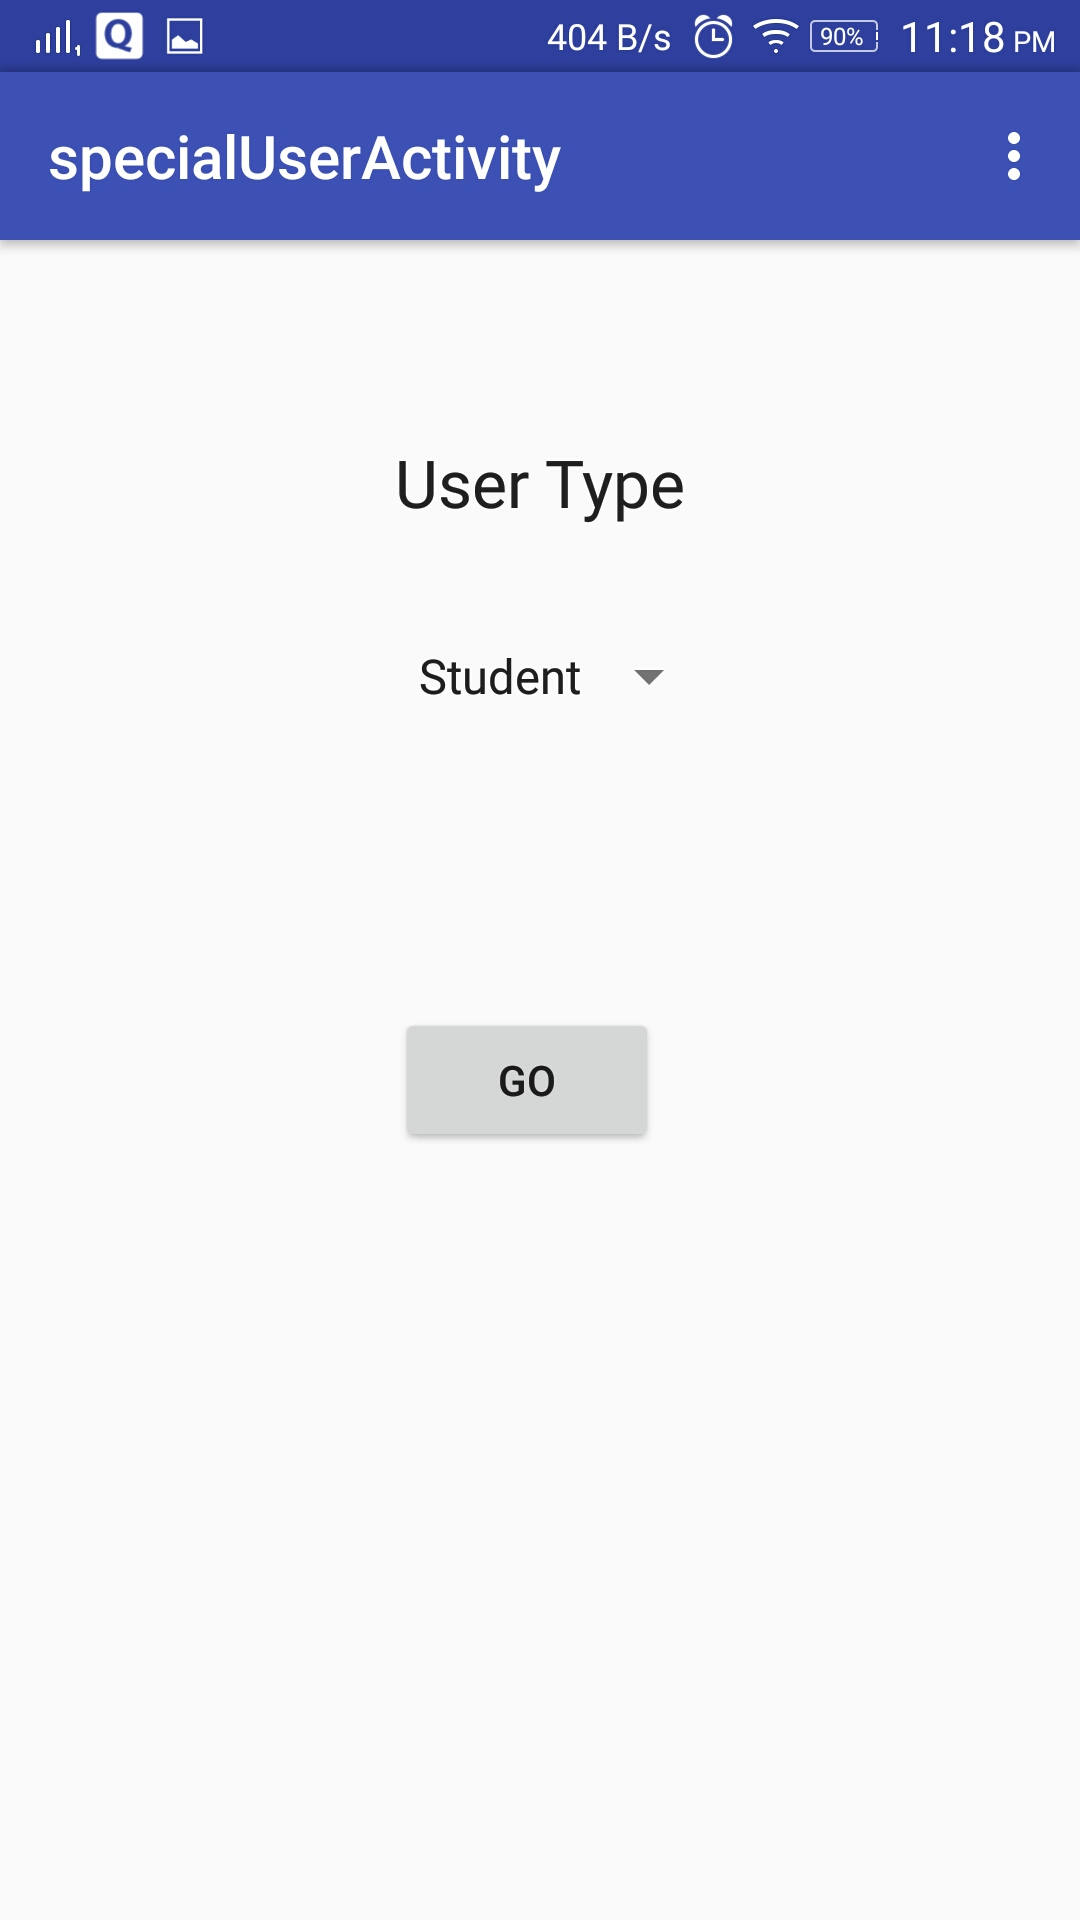
\includegraphics[width=0.5\textwidth]{specialuser.jpeg}
	\caption{Spinner to add new Users for Special User}
\end{figure}

\begin{figure}[!ht]
	\centering
	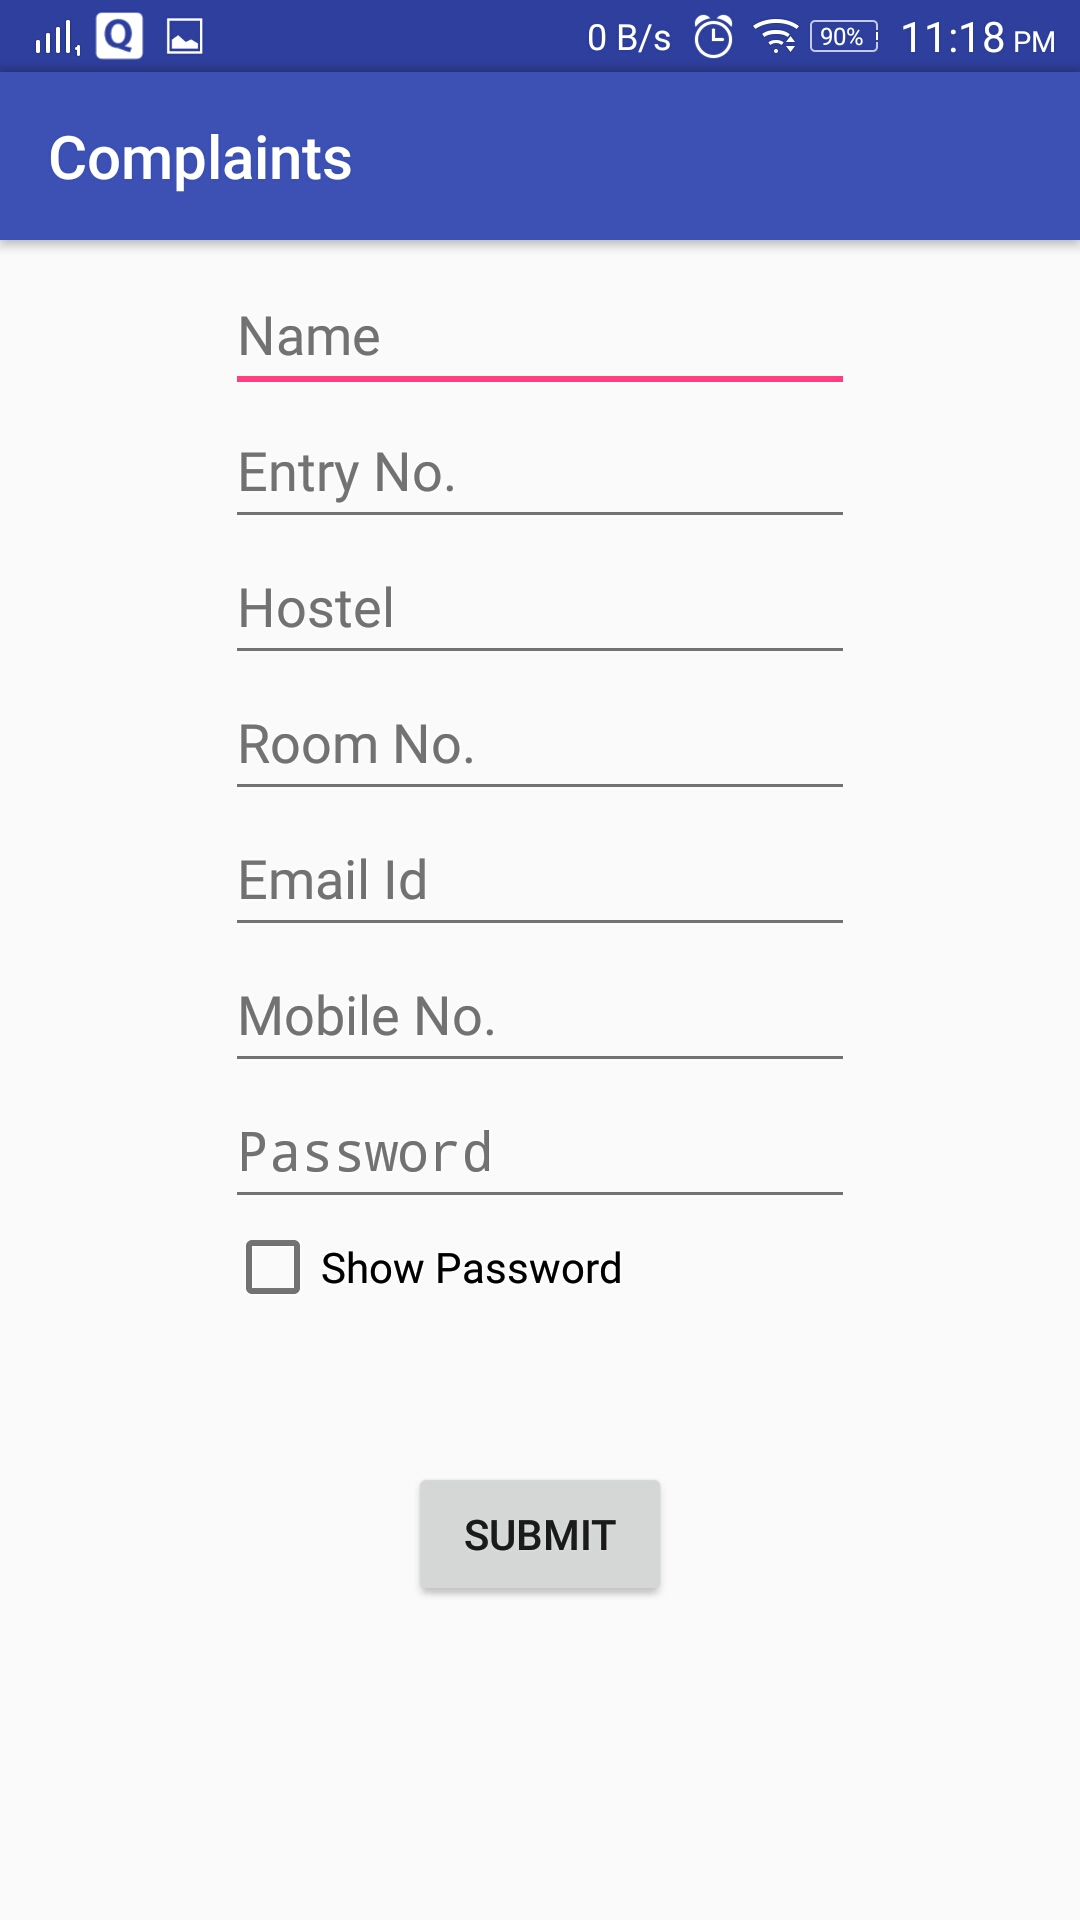
\includegraphics[width=0.5\textwidth]{addstudent.jpeg}
	\caption{Navigation Drawer for Special User}
\end{figure}
\begin{itemize}
    \item Form field with Name, Email, Hostel, Room No., Mobile No. required.
\end{itemize}


\section{Features}

\begin{itemize}
\item PHP is being used for backend server.
\item User information has been organised in different database tables.
\item Unique Complaint ticket ID is generated and assigned at server side when user submits a complaint.
\item Comment section is added where Problem submitter and technician can discuss about several issues related to the problem.
\item Problems by default has been sorted according to submission date within their categories.
\item Problem submitter can upload picture of the complaint for better insight for technician.
\item When a new Complaint is filed, related technician or authority gets notification on his/her mobile.
\item API has been developed in such a way that these can be used for Developing web application as well as Windows/ Iphone app.
\item 
\end{itemize}


\begin{figure}[!ht]
	\centering
	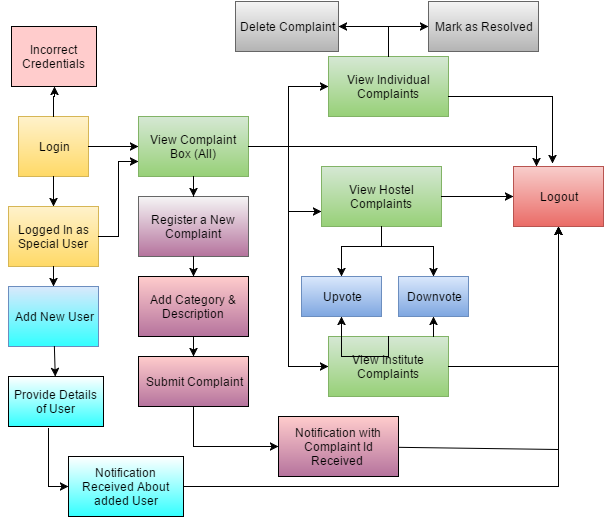
\includegraphics[scale=0.7]{workflow.png}
	\caption{Workflow of Application}
\end{figure}

\begin{figure}[!ht]
	\centering
	\includegraphics[scale=0.3]{erd.png}
	\caption{Entity Relationship Diagram}
\end{figure}

\begin{figure}[!ht]
	\centering
	\includegraphics[scale=0.6]{LoginAPI.png}
	\caption{Login API}
\end{figure}

\begin{figure}[!ht]
	\centering
	\includegraphics[scale=0.7]{NewComplaintAPI.png}
	\caption{Report Complaint API}
\end{figure}

\begin{figure}[!ht]
	\centering
	\includegraphics[scale=0.7]{UpvoteAPI.png}
	\caption{API to Upvote a public Question}
\end{figure}

\begin{figure}[!ht]
	\centering
	\includegraphics[scale=0.7]{DownvoteAPI.png}
	\caption{API to Downvote a public Question}
\end{figure}

\begin{figure}[!ht]
	\centering
	\includegraphics[scale=0.7]{AddUserAPI.png}
	\caption{API to add a new User}
\end{figure}

\begin{figure}[!ht]
	\centering
	\includegraphics[scale=0.7]{AllComplaintsAPI.png}
	\caption{API to fetch all complaints}
\end{figure}

\begin{figure}[!ht]
	\centering
	\includegraphics[scale=0.7]{HostelComplaintsAPI.png}
	\caption{API to fetch hostel complaints}
\end{figure}

\begin{figure}[!ht]
	\centering
	\includegraphics[scale=0.7]{InstituteComplaintsAPI.png}
	\caption{API to fetch Institute complaints}
\end{figure}

\begin{figure}[!ht]
	\centering
	\includegraphics[scale=0.7]{IndividualComplaintsAPI.png}
	\caption{API to fetch private complaints}
\end{figure}

\begin{figure}[!ht]
	\centering
	\includegraphics[scale=0.7]{DeleteComplaintAPI.png}
	\caption{API to Delete a complaint}
\end{figure}








\section{references}
\begin{itemize}
    \item http://stackoverflow.com
    \item http://youtube.com
    \item http://code.tutsplus.com
\end{itemize}

\end{document}
